% questions.tex —— 1983 年·全国卷（文科） · 题目内容片段（无答案）
% 由 tools/generate_projects.py 依来源总账自 1983/1983_数学真题_文_试题.md 生成，勿手改（改源 MD 后重跑）


\begin{gktip}
\textbf{来源说明}：本卷为 1983 年全国统一命题的\textbf{文科数学}卷（同年另有独立的理科卷，两份试卷题目不同），单页扫描（原卷页码第 22 页），全卷共 13 题，其中第 1—5 题为选择题。题面不含答案（答案由本库独立推导）。原卷按左、中、右三栏分栏排版，本文按题号 1—13 顺序转录，题面文字未作改动。

\textbf{题面说明}：第 6 题为填表题，原卷表格“图形名称”“图形”两行留空待填，本文照原卷保留空列。第 9、10、11、13 题依原卷配图重绘为 TikZ 矢量图。

\textbf{源注}：第 7 题第（1）问原卷根号只覆盖 $x+5$，对数式 $\log_2(36-x^2)$ 在根号之外；纯文本提取易误并为一个根号，本文按页面图像转录为 $y=\sqrt{x+5}\cdot\log_2(36-x^2)$。
\end{gktip}

\begin{question}
\gkti{1}在直角坐标系内，函数 $y=|x|$ 的图象\mbox{（　　）}

\begin{gkopts}(2)
\task A．关于坐标轴、原点都不对称
\task B．关于原点对称
\task C．关于 $x$ 轴对称
\task D．关于 $y$ 轴对称
\end{gkopts}

\end{question}
\begin{question}
\gkti{2}抛物线 $x^2+y=0$ 的焦点位于\mbox{（　　）}

\begin{gkopts}(2)
\task A．$y$ 轴的负半轴上
\task B．$y$ 轴的正半轴上
\task C．$x$ 轴的负半轴上
\task D．$x$ 轴的正半轴上
\end{gkopts}

\end{question}
\begin{question}
\gkti{3}两条异面直线，指的是\mbox{（　　）}

\begin{gkopts}(2)
\task A．在空间内不相交的两条直线
\task B．分别位于两个不同平面内的两条直线
\task C．某一平面内的一条直线和这个平面外的一条直线
\task D．不在同一平面内的两条直线
\end{gkopts}

\end{question}
\begin{question}
\gkti{4}对任何 $180^\circ<\alpha<360^\circ$，$\cos\dfrac{\alpha}{2}$ 的值等于\mbox{（　　）}

\begin{gkopts}(2)
\task A．$\sqrt{\dfrac{1+\cos\alpha}{2}}$
\task B．$\sqrt{\dfrac{1-\cos\alpha}{2}}$
\task C．$-\sqrt{\dfrac{1+\cos\alpha}{2}}$
\task D．$-\sqrt{\dfrac{1-\cos\alpha}{2}}$
\end{gkopts}

\end{question}
\begin{question}
\gkti{5}$0.3^2$，$\log_20.3$，$2^{0.3}$ 这三个数之间的大小顺序是\mbox{（　　）}

\begin{gkopts}(2)
\task A．$0.3^2<2^{0.3}<\log_20.3$
\task B．$0.3^2<\log_20.3<2^{0.3}$
\task C．$\log_20.3<0.3^2<2^{0.3}$
\task D．$\log_20.3<2^{0.3}<0.3^2$
\end{gkopts}

\end{question}
\begin{question}
\gkti{6}在平面直角坐标系内，表中的方程表示什么图形？画出这些图形。

\begin{center}
\begin{tabular}{cll}
\toprule
方程 & $x^2+y^2=2x$ & $x^2-y^2=0$ \\
\midrule
图形名称 &  &  \\
图形 &  &  \\
\bottomrule
\end{tabular}
\end{center}

\end{question}
\begin{question}
\gkti{7}

（1） 求函数 $y=\sqrt{x+5}\log_2(36-x^2)$ 的定义域。

（2） 一个小组共有 10 名同学，其中 4 名是女同学，6 名是男同学。要从小组内选出 3 名代表，其中至少有 1 名女同学，求一共有多少种选法。

\end{question}
\begin{question}
\gkti{8}已知复数 $z=\cos\alpha+\mathrm i\sin\alpha$，求证：$z^3+\dfrac{1}{z^3}=2\cos3\alpha$。

\Needspace{0.4\textheight}
\end{question}
\begin{question}
\gkti{9}在圆心为 $O$、半径为常数 $R$ 的半圆板内画内接矩形（如图），当矩形的长和宽各取多少时，矩形的面积最大？求出这个最大面积。
\nopagebreak[4]
\begin{center}% 1983 年全国卷（文科）第 9 题：半圆板内接矩形——底边落在直径上、关于过圆心 O 的竖直线对称，矩形上边两顶点在弧上；O 为圆心，R 为半径，图下方以双向箭头标出半径 R（按源卷布局）
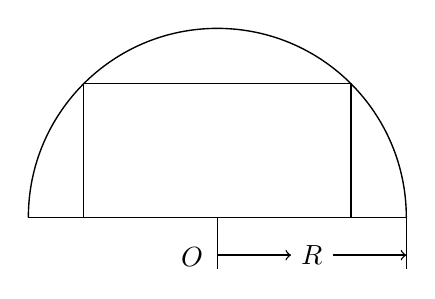
\begin{tikzpicture}[scale=1.2, line width=0.5pt,
  every node/.style={inner sep=1.5pt}]
  % 直径与半圆弧（圆心在原点，半径 2）
  \draw (-2,0) -- (2,0);
  \draw (-2,0) arc (180:0:2);
  % 内接矩形：半底 √2、高 √2（即面积最大时的长宽）
  \draw (-1.4142,0) -- (-1.4142,1.4142) -- (1.4142,1.4142) -- (1.4142,0);
  % 圆心 O 与右端点处的短竖线
  \draw (0,0) -- (0,-0.55);
  \draw (2,0) -- (2,-0.55);
  % 半径 R 的双向箭头（中间留白写 R）
  \draw[->] (0,-0.40) -- (0.78,-0.40);
  \draw[->] (1.22,-0.40) -- (2,-0.40);
  \node at (1,-0.40) {$R$};
  \node[anchor=east] at (-0.10,-0.42) {$O$};
\end{tikzpicture}
\end{center}
\nopagebreak[4]
\Needspace{0.4\textheight}
\end{question}
\begin{question}
\gkti{10}如图，地平面上有一旗杆 $OP$，为了测得它的高度 $h$，在地面上选一基线 $AB$，$AB=20$ 米，在 $A$ 点处测得 $P$ 点的仰角 $\angle OAP=30^\circ$，在 $B$ 点处测得 $P$ 点的仰角 $\angle OBP=45^\circ$，又测得 $\angle AOB=60^\circ$，求旗杆的高度 $h$（结果可以保留根号）。
\nopagebreak[4]
\begin{center}% 1983 年全国卷（文科）第 10 题：地平面上旗杆 OP（高 h），基线 AB=20 米，A 处仰角 ∠OAP=30°、B 处仰角 ∠OBP=45°、∠AOB=60°；AO 为水平辅助线（虚线），PO 竖直（按源卷布局）
\begin{tikzpicture}[scale=0.8, line width=0.5pt,
  every node/.style={inner sep=1.5pt}]
  \coordinate (A) at (-6.35,0);
  \coordinate (O) at (0,0);
  \coordinate (P) at (0,3.90);
  \coordinate (B) at (-2.40,-3.10);
  \draw (A) -- (P);
  \draw (A) -- (B);
  \draw (B) -- (O);
  \draw (B) -- (P);
  \draw (O) -- (P);
  \draw[dashed] (A) -- (O);
  % 三个角的弧线与度数标注
  \draw (A) ++(0:0.85) arc (0:31.6:0.85);
  \node at (-5.05,0.62) {$30^\circ$};
  \draw (O) ++(180:0.75) arc (180:232:0.75);
  \node at (-1.05,-0.58) {$60^\circ$};
  \draw (B) ++(52:0.95) arc (52:71:0.95);
  \node at (-1.60,-1.66) {$45^\circ$};
  % 高度与基线标注
  \node[anchor=west] at (0.16,1.95) {$h$};
  \node at (-5.30,-1.90) {20 米};
  % 顶点标注
  \node[anchor=east] at (-6.45,0) {$A$};
  \node[anchor=south] at (0,4.02) {$P$};
  \node[anchor=west] at (0.16,-0.28) {$O$};
  \node[anchor=north] at (-2.40,-3.34) {$B$};
\end{tikzpicture}
\end{center}
\nopagebreak[4]
\Needspace{0.4\textheight}
\end{question}
\begin{question}
\gkti{11}如图，已知一块直角三角形板 $ABC$ 的 $BC$ 边在平面 $\alpha$ 内，$\angle ABC=60^\circ$，$\angle ACB=30^\circ$，$BC=24\ \mathrm{cm}$，$A$ 点在平面 $\alpha$ 内的射影为 $N$，$AN=9\ \mathrm{cm}$。求以 $A$ 为顶点的三棱锥 $A\text{-}NBC$ 的体积（结果可以保留根号）。
\nopagebreak[4]
\begin{center}% 1983 年全国卷（文科）第 11 题：直角三角形板 ABC 的 BC 边在平面 α 内，A 在 α 内的射影为 N；连 AB、AC、AN、NB、NC、BC，其中 NC 及 α 后边被面 ANC 遮住的一段画虚线（按源卷布局）
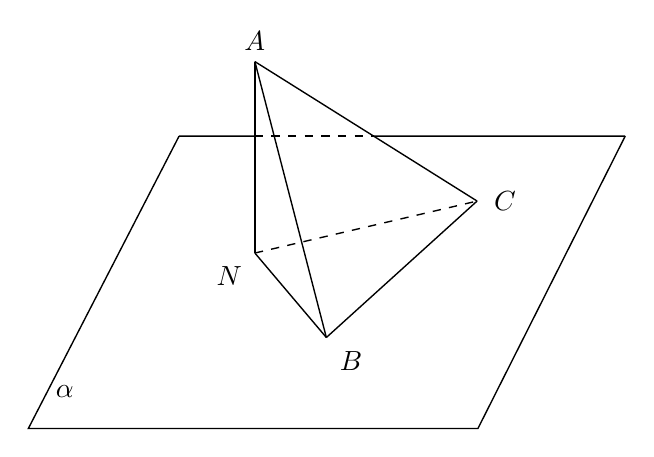
\begin{tikzpicture}[scale=1.1, line width=0.5pt,
  every node/.style={inner sep=1.5pt}]
  % 平面 α 的平行四边形（后边 TL—TR 中段被遮挡，画虚线）
  \coordinate (TL) at (0.90,3.25);
  \coordinate (TR) at (6.05,3.25);
  \coordinate (BR) at (4.35,-0.125);
  \coordinate (BL) at (-0.84,-0.125);
  \draw (TR) -- (BR) -- (BL) -- (TL);
  \draw (TL) -- (1.775,3.25);
  \draw[dashed] (1.775,3.25) -- (3.145,3.25);
  \draw (3.145,3.25) -- (TR);
  % 顶点
  \coordinate (A) at (1.775,4.11);
  \coordinate (N) at (1.775,1.90);
  \coordinate (C) at (4.34,2.50);
  \coordinate (B) at (2.60,0.925);
  % 棱
  \draw (A) -- (N);
  \draw (A) -- (B);
  \draw (A) -- (C);
  \draw (N) -- (B);
  \draw (B) -- (C);
  \draw[dashed] (N) -- (C);
  % 标注
  \node[anchor=south] at (1.775,4.18) {$A$};
  \node[anchor=north east] at (1.68,1.80) {$N$};
  \node[anchor=west] at (4.48,2.50) {$C$};
  \node[anchor=north west] at (2.70,0.82) {$B$};
  \node at (-0.42,0.30) {$\alpha$};
\end{tikzpicture}
\end{center}
\nopagebreak[4]
\end{question}
\begin{question}
\gkti{12}一个等比数列有三项，如果把第二项加上 4，那么所得的三项就成为等差数列；如果再把等差数列的第三项加上 32，那么所得的三项又成等比数列。求原来的等比数列。

\Needspace{0.4\textheight}
\end{question}
\begin{question}
\gkti{13}如图，已知两条直线 $L_1:2x-3y+2=0$，$L_2:3x-2y+3=0$。有一动圆（圆心和半径都在变动）与 $L_1$、$L_2$ 都相交，并且 $L_1$、$L_2$ 被截在圆内的两条线段长度分别是定值 26，24。求圆心 $M$ 的轨迹方程，并说出轨迹的名称。
\nopagebreak[4]
\begin{center}% 1983 年全国卷（文科）第 13 题：动圆（圆心 M）与两条定直线 L1、L2 都相交，L1、L2 都过 x 轴上原点左侧一点；两条直线在图中按源卷画成 L1 陡、L2 缓（与方程斜率恰相反，源图为示意图），圆心 M 在圆内偏右（按源卷布局）
\begin{tikzpicture}[scale=1, line width=0.5pt,
  every node/.style={inner sep=1.5pt}]
  % 坐标轴
  \draw[->] (-2.2,0) -- (5.6,0) node[below] {$x$};
  \draw[->] (0,-1.8) -- (0,4.6) node[left] {$y$};
  \node[anchor=north east] at (-0.12,-0.10) {$O$};
  % 两条定直线（都过 (-0.9,0)）
  \draw (-1.60,-0.84) -- (3.20,4.92) node[above right] {$L_1$};
  \draw (-1.50,-0.232) -- (5.00,2.277) node[above right] {$L_2$};
  % 动圆与圆心 M
  \draw (2.5,1.85) circle (1.6);
  \fill (2.5,1.85) circle (0.055);
  \node[anchor=west] at (2.62,1.85) {$M$};
\end{tikzpicture}
\end{center}
\nopagebreak[4]

\end{question}